%%%%%%%%%%%%%%%%%%%%%%%%%%%%%%%%%%%%%%%%%
% Programming/Coding Assignment
% LaTeX Template
%
% This template has been downloaded from:
% http://www.latextemplates.com
%
% Original author:
% Ted Pavlic (http://www.tedpavlic.com)
%
% Note:
% The \lipsum[#] commands throughout this template generate dummy text
% to fill the template out. These commands should all be removed when 
% writing assignment content.
%
% This template uses a Perl script as an example snippet of code, most other
% languages are also usable. Configure them in the "CODE INCLUSION 
% CONFIGURATION" section.
%
%%%%%%%%%%%%%%%%%%%%%%%%%%%%%%%%%%%%%%%%%

%----------------------------------------------------------------------------------------
%	PACKAGES AND OTHER DOCUMENT CONFIGURATIONS
%----------------------------------------------------------------------------------------

\documentclass{article}

\usepackage{fancyhdr} % Required for custom headers
\usepackage{lastpage} % Required to determine the last page for the footer
\usepackage{extramarks} % Required for headers and footers
\usepackage[usenames,dvipsnames]{color} % Required for custom colors
\usepackage{graphicx} % Required to insert images
\usepackage{subcaption}
\usepackage{listings} % Required for insertion of code
\usepackage{courier} % Required for the courier font
\usepackage{lipsum} % Used for inserting dummy 'Lorem ipsum' text into the template
\usepackage{amsmath}
\usepackage{amssymb}
\usepackage{amsthm}


% Margins
\topmargin=-0.45in
\evensidemargin=0in
\oddsidemargin=0in
\textwidth=6.5in
\textheight=9.0in
\headsep=0.25in

\linespread{1.1} % Line spacing

% Set up the header and footer
\pagestyle{fancy}
\lhead{\hmwkAuthorName} % Top left header
\chead{\hmwkClass\ (\hmwkClassTime): \hmwkTitle} % Top center head
%\rhead{\firstxmark} % Top right header
\lfoot{\lastxmark} % Bottom left footer
\cfoot{} % Bottom center footer
\rfoot{Page\ \thepage\ of\ \protect\pageref{LastPage}} % Bottom right footer
\renewcommand\headrulewidth{0.4pt} % Size of the header rule
\renewcommand\footrulewidth{0.4pt} % Size of the footer rule

\setlength\parindent{0pt} % Removes all indentation from paragraphs

%----------------------------------------------------------------------------------------
%	CODE INCLUSION CONFIGURATION
%----------------------------------------------------------------------------------------

\definecolor{MyDarkGreen}{rgb}{0.0,0.4,0.0} % This is the color used for comments
\lstloadlanguages{Perl} % Load Perl syntax for listings, for a list of other languages supported see: ftp://ftp.tex.ac.uk/tex-archive/macros/latex/contrib/listings/listings.pdf
\lstset{language=Perl, % Use Perl in this example
        frame=single, % Single frame around code
        basicstyle=\small\ttfamily, % Use small true type font
        keywordstyle=[1]\color{Blue}\bf, % Perl functions bold and blue
        keywordstyle=[2]\color{Purple}, % Perl function arguments purple
        keywordstyle=[3]\color{Blue}\underbar, % Custom functions underlined and blue
        identifierstyle=, % Nothing special about identifiers                                         
        commentstyle=\usefont{T1}{pcr}{m}{sl}\color{MyDarkGreen}\small, % Comments small dark green courier font
        stringstyle=\color{Purple}, % Strings are purple
        showstringspaces=false, % Don't put marks in string spaces
        tabsize=5, % 5 spaces per tab
        %
        % Put standard Perl functions not included in the default language here
        morekeywords={rand},
        %
        % Put Perl function parameters here
        morekeywords=[2]{on, off, interp},
        %
        % Put user defined functions here
        morekeywords=[3]{test},
       	%
        morecomment=[l][\color{Blue}]{...}, % Line continuation (...) like blue comment
        numbers=left, % Line numbers on left
        firstnumber=1, % Line numbers start with line 1
        numberstyle=\tiny\color{Blue}, % Line numbers are blue and small
        stepnumber=5 % Line numbers go in steps of 5
}

% Creates a new command to include a perl script, the first parameter is the filename of the script (without .pl), the second parameter is the caption
\newcommand{\perlscript}[2]{
\begin{itemize}
\item[]\lstinputlisting[caption=#2,label=#1]{#1.pl}
\end{itemize}
}

%----------------------------------------------------------------------------------------
%	DOCUMENT STRUCTURE COMMANDS
%	Skip this unless you know what you're doing
%----------------------------------------------------------------------------------------

% Header and footer for when a page split occurs within a problem environment
\newcommand{\enterProblemHeader}[1]{
%\nobreak\extramarks{#1}{#1 continued on next page\ldots}\nobreak
%\nobreak\extramarks{#1 (continued)}{#1 continued on next page\ldots}\nobreak
}

% Header and footer for when a page split occurs between problem environments
\newcommand{\exitProblemHeader}[1]{
%\nobreak\extramarks{#1 (continued)}{#1 continued on next page\ldots}\nobreak
%\nobreak\extramarks{#1}{}\nobreak
}

\setcounter{secnumdepth}{0} % Removes default section numbers
\newcounter{homeworkProblemCounter} % Creates a counter to keep track of the number of problems
\setcounter{homeworkProblemCounter}{0}

\newcommand{\homeworkProblemName}{}
\newenvironment{homeworkProblem}[1][Part \arabic{homeworkProblemCounter}]{ % Makes a new environment called homeworkProblem which takes 1 argument (custom name) but the default is "Problem #"
\stepcounter{homeworkProblemCounter} % Increase counter for number of problems
\renewcommand{\homeworkProblemName}{#1} % Assign \homeworkProblemName the name of the problem
\section{\homeworkProblemName} % Make a section in the document with the custom problem count
\enterProblemHeader{\homeworkProblemName} % Header and footer within the environment
}{
\exitProblemHeader{\homeworkProblemName} % Header and footer after the environment
}

\newcommand{\problemAnswer}[1]{ % Defines the problem answer command with the content as the only argument
\noindent\framebox[\columnwidth][c]{\begin{minipage}{0.98\columnwidth}#1\end{minipage}} % Makes the box around the problem answer and puts the content inside
}

\newcommand{\homeworkSectionName}{}
\newenvironment{homeworkSection}[1]{ % New environment for sections within homework problems, takes 1 argument - the name of the section
\renewcommand{\homeworkSectionName}{#1} % Assign \homeworkSectionName to the name of the section from the environment argument
\subsection{\homeworkSectionName} % Make a subsection with the custom name of the subsection
\enterProblemHeader{\homeworkProblemName\ [\homeworkSectionName]} % Header and footer within the environment
}{
\enterProblemHeader{\homeworkProblemName} % Header and footer after the environment
}

%----------------------------------------------------------------------------------------
%	NAME AND CLASS SECTION
%----------------------------------------------------------------------------------------

\newcommand{\hmwkTitle}{Assignment\ \#$4$} % Assignment title
\newcommand{\hmwkDueDate}{Monday,\ April\ 2,\ 2018} % Due date
\newcommand{\hmwkClass}{CSC411} % Course/class
\newcommand{\hmwkClassTime}{L0101} % Class/lecture time
\newcommand{\hmwkAuthorName}{Yifei Dong, Zifei Han} % Your name

%----------------------------------------------------------------------------------------
%	TITLE PAGE
%----------------------------------------------------------------------------------------

\title{
\vspace{2in}
\textmd{\textbf{\hmwkClass:\ \hmwkTitle}}\\
\normalsize\vspace{0.1in}\small{Due\ on\ \hmwkDueDate}\\
\vspace{0.1in}
\vspace{3in}
}

\author{\textbf{\hmwkAuthorName}}
\date{April 2, 2018} % Insert date here if you want it to appear below your name

%----------------------------------------------------------------------------------------

\begin{document}

\maketitle
\clearpage
%----------------------------------------------------------------------------------------
%	PROBLEM 1
%----------------------------------------------------------------------------------------

% To have just one problem per page, simply put a \clearpage after each problem

\begin{homeworkProblem}

\noindent \textit{Environment description}\\
1. The grid is represented by a 2D array, displayed as 3x3 grid.  Empty grids are represented with ".", while first and second player's move is represented with symbol "x" and "o" consecutively. \\

2. Attribute 'turn" represents who's turn is it. When it's player1, turn equals "1" and action will show as "x" on the grid; When it's player2, turn equals "2" and action will show as "o" on the grid.\\

3. Attribute "done" represents if the game is over. If done is false, then it's not over. If done is true, then one of the player wins or there's a tie. \\

4. Create a new environment, and play a game of Tic-Tac-Toe against yourself by calling the step(), and render() methods. Display the text output in picture below.

\begin{verbatim}
env.render()
...
...
...
====
env.step(4)
(array([0, 0, 0, 0, 1, 0, 0, 0, 0]), 'valid', False)
env.render()
...
.x.
...
====
env.step(0)
(array([2, 0, 0, 0, 1, 0, 0, 0, 0]), 'valid', False)
env.render()
o..
.x.
...
====
env.step(6)
(array([2, 0, 0, 0, 1, 0, 1, 0, 0]), 'valid', False)
env.render()
o..
.x.
x..
====
env.step(2)
(array([2, 0, 2, 0, 1, 0, 1, 0, 0]), 'valid', False)
env.render()
o.o
.x.
x..
====
env.step(1)
(array([2, 1, 2, 0, 1, 0, 1, 0, 0]), 'valid', False)
env.render()
oxo
.x.
x..
====
env.step(8)
(array([2, 1, 2, 0, 1, 0, 1, 0, 2]), 'valid', False)
env.render()
oxo
.x.
x.o
====
env.step(7)
(array([2, 1, 2, 0, 1, 0, 1, 1, 2]), 'win', True)
\end{verbatim}




\end{homeworkProblem}
\clearpage
%----------------------------------------------------------------------------------------
%	PROBLEM 2
%----------------------------------------------------------------------------------------

\begin{homeworkProblem}
\noindent \textit{Policy Implementation}
\subsection{Part A}
\begin{lstlisting}
class Policy(nn.Module):
    """
    The Tic-Tac-Toe Policy
    """
    def __init__(self, input_size=27, hidden_size=64, output_size=9):
        super(Policy, self).__init__()
        self.layer = nn.Sequential(
            nn.Linear(input_size, hidden_size),
            nn.ReLU(),
            nn.Linear(hidden_size, output_size),
        )        

    def forward(self, x):
        x = self.layer(x)
        x = F.softmax(x, dim=-1)
        return x
\end{lstlisting}

\subsection{Part B}
There are 9 grids, and 3 possible values in each grid. In total there are 27 possibilities which forms a list of 27 elements that is the output from select\_action. \\
The first 9 values of the output list from select\_action is the indicator if the grids are empty. The second 9 values form the output list is the indicator if the grid has an "x" on it. The last 9 values  is the indicator if the grid has an "o" on it. 

\begin{lstlisting}
Example 1: 
   When all the grid is empty, the first 9 values all have value 1,
   indicates empty grids. 
array([0, 0, 0, 0, 0, 0, 0, 0, 0])
state value listed below:
    1     1     1     1     1     1     1     1     1    
    0     0     0     0     0     0     0     0     0
    0     0     0     0     0     0     0     0     0
[torch.FloatTensor of size 1x27]

Example 2:
array([0, 0, 2, 1, 0, 0, 0, 0, 0])
state value listed below:
    1     1     0     0     1     1     1     1     1
    0     0     0     1     0     0     0     0     0
    0     0     1     0     0     0     0     0     0
[torch.FloatTensor of size 1x27]
\end{lstlisting}


\subsection{Part C}
The output of this policy is a 9-dimensional vector. The value in each output represents the possibility each grid is the next move. The index of the highest value in the output is the index of the next move.\\

This policy is stochastic.\\




\end{homeworkProblem}
\clearpage
%----------------------------------------------------------------------------------------
%	PROBLEM 3
%----------------------------------------------------------------------------------------

\begin{homeworkProblem}

\subsection{Part A}
\begin{lstlisting}
def compute_returns(rewards, gamma=1.0):
    """
    Compute returns for each time step, given the rewards
      @param rewards: list of floats, where rewards[t] is the reward
                      obtained at time step t
      @param gamma: the discount factor
      @returns list of floats representing the episode's returns
          G_t = r_t + \gamma r_{t+1} + \gamma^2 r_{t+2} + ... 

    >>> compute_returns([0,0,0,1], 1.0)
    [1.0, 1.0, 1.0, 1.0]
    >>> compute_returns([0,0,0,1], 0.9)
    [0.7290000000000001, 0.81, 0.9, 1.0]
    >>> compute_returns([0,-0.5,5,0.5,-10], 0.9)
    [-2.5965000000000003, -2.8850000000000002, -2.6500000000000004, -8.5, -10.0]
    """
    size = len(rewards)
    result = [0] * size
    i = size - 1
    while i >= 0:
        if i == size - 1:
            result[i] = float(rewards[i])
        else:
            result[i] = rewards[i] + gamma * result[i+1]
        i -= 1
    return result
\end{lstlisting}


\subsection{Part B}
We cannot compute backward pass and update weights while the game is not done, because we don't have a definite reward until the game is done. While the game is still playing, we can only know if a move is valid but cannot know whether the move is a good or bad one since we don't know the result of the game. That's why the reward won't be definite until the game is done.


\end{homeworkProblem}
\clearpage

%----------------------------------------------------------------------------------------
%	PROBLEM 4
%----------------------------------------------------------------------------------------

\begin{homeworkProblem}
\subsection{Part A}
\begin{lstlisting}
def get_reward(status):
    """Returns a numeric given an environment status."""
    return {
            Environment.STATUS_VALID_MOVE  : 10, 
            Environment.STATUS_INVALID_MOVE: -10,
            Environment.STATUS_WIN         : 50,
            Environment.STATUS_TIE         : -5,
            Environment.STATUS_LOSE        : -50
    }[status]
\end{lstlisting}

\subsection{Part B}
Explain the choices that we made in 4(a): 
1. Valid move and invalid move contradict each other. Therefore, a valid move is rewarded 10 points and an invalid move is penalized -10 points. \\
2. Win, Loose and Tie are a group of status. For win we reward 50 points, while lose is penalized the same amount of points (-50). As for tie, it's (-5) reward points because it's better than lose. But it's still not something we want. 3. The magnitude of the rewards is selected based on the importance of the status. Win is a better result than valid move, therefore it has 5 times the score as valid move. Others are scaled accordingly. \\

We have also tested among several different sets of values to see which one leads to better performance of the agent.




\end{homeworkProblem}
\clearpage

%----------------------------------------------------------------------------------------
%	PROBLEM 5
%----------------------------------------------------------------------------------------

\begin{homeworkProblem}

\subsection{Part A}
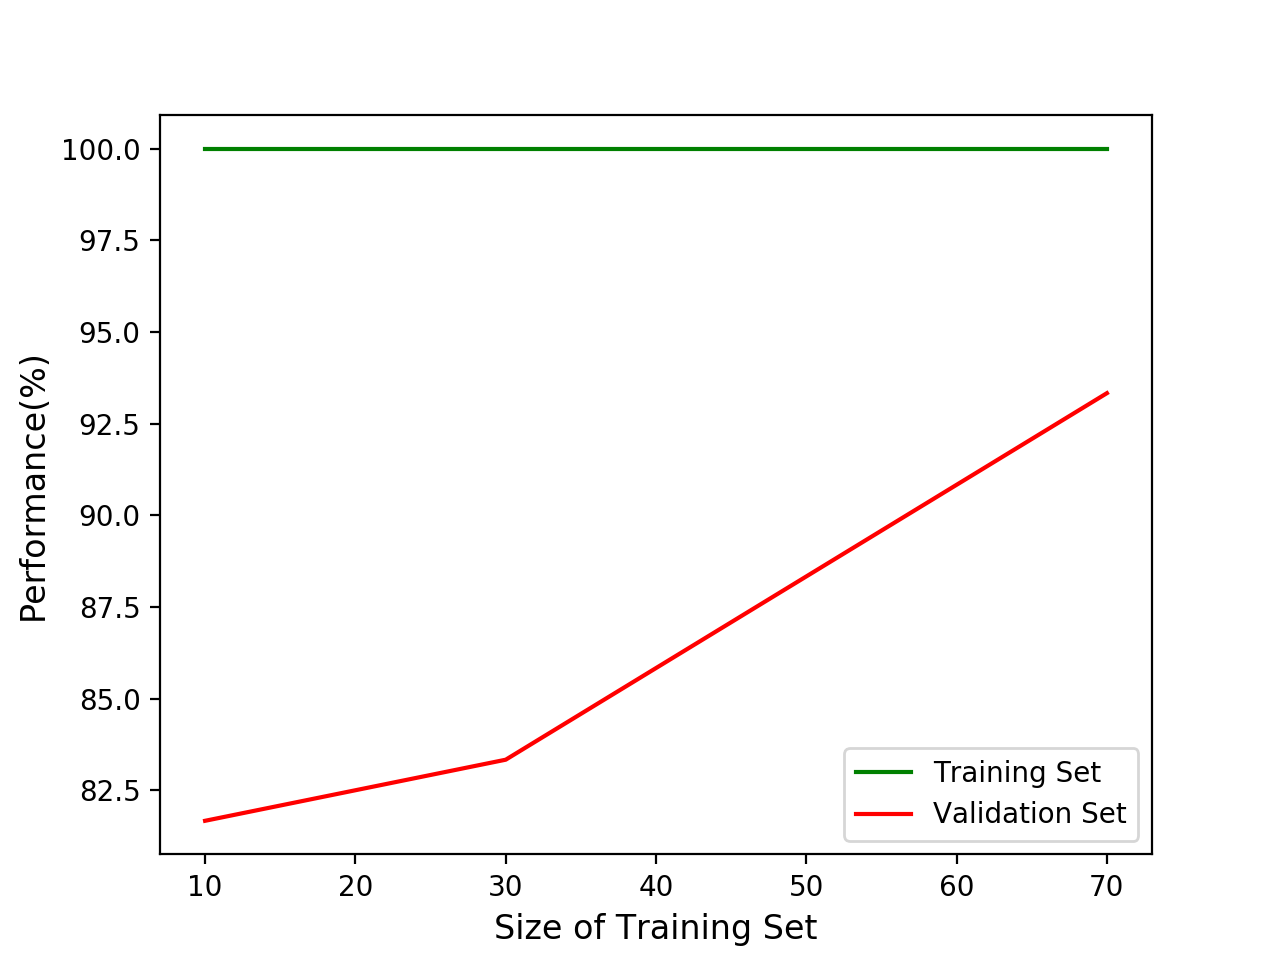
\includegraphics[scale = 0.8]{part5.png}\\
We changed gamma to 0.70. We tried other hyper parameters like 0.9, 0.8, 0.75, 0.6. Among different gamma values, 0.70 gives the best performance.
\clearpage

\subsection{Part B}
We tried three hidden units number and plot the learning curve of it. \\
1. Hidden Unit Number = 30. \hspace{2cm} 2. Hidden Unit Number = 120.\\
\includegraphics[scale = 0.45]{part5b30.png}
\includegraphics[scale = 0.45]{part5b120.png}\\
3. Hidden Unit Number = 240.\\
\includegraphics[scale = 0.45]{part5b240.png}\\

Conclusion: Too large or too small hidden unit length does not perform as well as 64 hidden unit length. The one with larger number of hidden units performed worse.
\clearpage
\subsection{Part C}
We tried two ways to analyze when our algorithm learn to stop playing invalid moves. \\

1. Firstly, by plotting the invalid move against number of episodes. The resulted graph is shown below. We can see that the number of invalid moves has dropped significantly as iterations increases and converges to zero at around 35000 episodes and on-wards. \\
\includegraphics[scale = 0.7]{part5c1.png}\\

2. Secondly we identified decrease of invalid move by analyzing the learning curve in part(a). The slope became more smooth at 35000 episode and it is increasing in a steady path, which means that we stopped getting invalid moves. 
\subsection{Part D}
1. Play 100 Games against Random. \\
From the result of fcuntion \textbf{games\_play\_against\_random(policy, env)}.\\
The agent won 94 times, lost 5 times, and tied 1 time.\\

2. Display five games that our trained agent plays against the random policy. Explain any strategies that you think your agent has learned.
\begin{lstlisting}
Game1:
...
.xo
...
====
...
.xo
o.x
====
x..
.xo
o.x
====
******************
Game2:
...
.xo
...
====
x..
.xo
..o
====
x.x
.xo
.oo
====
x.x
.xo
xoo
====
******************
Game3:
o..
.x.
...
====
o.x
.x.
o..
====
oox
xx.
o..
====
oox
xxx
o..
====
******************
Game4:
...
.x.
..o
====
..x
.xo
..o
====
..x
.xo
x.o
====
******************
Game5:
o..
.x.
...
====
o.x
ox.
...
====
o.x
ox.
x..
====
******************
\end{lstlisting}
Conclusion: there are are several strategies that we believe the agent has learned. \\
1. Always start in the middle of the grid. The first move is always the middle one. \\
2. The second move of "x" should always be on one of the corners that gives more paths to win. \\
3. The third move of "x" is to aim to block "o" to win, as we called is as "blocking move".
\end{homeworkProblem}
\clearpage

%----------------------------------------------------------------------------------------
%	PROBLEM 6
%----------------------------------------------------------------------------------------

\begin{homeworkProblem}
We compute the learning rate form 100 random games for each episode. Each iteration of episode we used the current policy to play 100 games and calculate the win/loose rate. The result over episode iteration is shown in graph below: 

\includegraphics[scale = 0.7]{part6.png}\\

Conclusion:
We can see that the win rate has improved from around 60\% to 90\% over 50000 episodes. The tie rate is always low and  decreasing slowly and the loss rate decreased from around 25\% to around 0.2\%.
\end{homeworkProblem}
\clearpage

%----------------------------------------------------------------------------------------
%	PROBLEM 7
%----------------------------------------------------------------------------------------

\begin{homeworkProblem}
\noindent \textit{First Move Analysis}

1. For the final trained model, $\pi(a|s_0)$ - the learned distribution over the first move is shown as below: 
\begin{lstlisting}
Columns 0 to 5 
 3.5264e-05  4.9005e-07  4.5341e-05  3.7189e-08  9.9972e-01  4.5391e-08

Columns 6 to 8 
 5.0122e-06  1.7546e-04  2.3234e-05
\end{lstlisting}
From the result we can see that the value at index 4, which is the indicator of the middle gird has significantly higher value than other values. \\

2. Conclusion: Our Modal has learned that we should always start in the middle (i.e: the first "x" should always be at index 4, the middle of the grid.) \\
I think it make sense because by landing the first move in the middle, the player1 has the most chance to win. \\

3. To explore how the distribution over the first move has changed throughout training, we plotted nine graphs for each of the index in $\pi(a|s_0)$ in order to show how the distribution has changed:

\includegraphics[scale=0.35]{p7m0.png}
\includegraphics[scale=0.35]{p7m1.png}
\includegraphics[scale=0.35]{p7m2.png}\\
\includegraphics[scale=0.35]{p7m3.png}
\includegraphics[scale=0.35]{p7m4.png}
\includegraphics[scale=0.35]{p7m5.png}\\
\includegraphics[scale=0.35]{p7m6.png}
\includegraphics[scale=0.35]{p7m7.png}
\includegraphics[scale=0.35]{p7m8.png}\\

Conclusion: The values fluctuates at the beginning but become more stable at the end. The value at index 4 is increasing and all other values at other indexes are decreasing as number of episode increases. 


\end{homeworkProblem}
\clearpage

%----------------------------------------------------------------------------------------
%	PROBLEM 8
%----------------------------------------------------------------------------------------

\begin{homeworkProblem}
\noindent \textit{Limitations}\\

One of the mistakes the agent make is that the agent did not predict or consider the possible moves of the opponent before the agent decides his moves.\\

Also, the agent does not play the optimal move sometimes. For example:
\begin{verbatim}
.x.
...
.o.
====
.x.
.x.
oo.
====
\end{verbatim}
The agent shouldn't put 'x' at position [4] at his second step since there's already an 'o' at position [7] and position [1][4][7] cannot provide a 'x' row anymore.


\end{homeworkProblem}
\clearpage

%----------------------------------------------------------------------------------------


\end{document}